%%%%%%%%%%%%%%%%%%%%%%%%%%%%%%%%%%%%%%%%%%%%%%%%%%%%%%%%%%%%%%%%%%%%%%%%%%%%%%%%%%
\begin{frame}[fragile]\frametitle{}
\begin{center}
{\Large Linear Algebra - Python Implementation}
\end{center}
\end{frame}

%%%%%%%%%%%%%%%%%%%%%%%%%%%%%%%%%%%%%%%%%%%%%%%%%%%%%%%%%%%%%%%%%%%%%%%%
\begin{frame}[fragile]\frametitle{Vectors}
\begin{itemize}
\item If we have data of people with 3 attributes
\item  Heights, weights, and ages
\item Each data point is in 3-D space with (height,  weight,  age) basis.
\item In python, we can use list
\end{itemize}
\begin{lstlisting}
height_weight_age = [70,  # inches,
                     170, # pounds,
                     40 ] # years
\end{lstlisting}
\end{frame}

%%%%%%%%%%%%%%%%%%%%%%%%%%%%%%%%%%%%%%%%%%%%%%%%%%%%%%%%%%%%%%%%%%%%%%%%
\begin{frame}[fragile]\frametitle{Vectors}
\begin{itemize}
\item lists are ok to represent vectors as storage, but not appropriate for operations
\item Why?
\item Whats list additions?
\item Whats vector addition?
\end{itemize}
\end{frame}

%%%%%%%%%%%%%%%%%%%%%%%%%%%%%%%%%%%%%%%%%%%%%%%%%%%%%%%%%%%%%%%%%%%%%%%%
\begin{frame}[fragile]\frametitle{Vector Addition}
\begin{itemize}
\item We'll frequently need to add two vectors. 
\item Vectors add component-wise.
\item Resultant first element is  $v[0] + w[0]$ , 
\item Resultant second element is  $v[1] + w[1]$ , and so on. 
\item If they're not the same length,  not allowed to add them.
\end{itemize}
\begin{center}
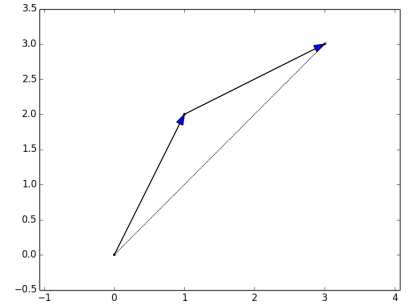
\includegraphics[width=0.5\linewidth]{vecadd}
\end{center}
\end{frame}

%%%%%%%%%%%%%%%%%%%%%%%%%%%%%%%%%%%%%%%%%%%%%%%%%%%%%%%%%%%%%%%%%%%%%%%%
\begin{frame}[fragile]\frametitle{Vector Addition}
\begin{itemize}
\item Implement vector addition
\item Hint: `zip' two vectors and use List Comprehension
\end{itemize}
\begin{lstlisting}
def vector_add(v, w):
	:
	return [...]
vv = [ 1, 2,3]
ww = [3,2,1]
result = vector_add(vv,ww)
print("Vector Addition {}".format(result))
\end{lstlisting}
\end{frame}


%%%%%%%%%%%%%%%%%%%%%%%%%%%%%%%%%%%%%%%%%%%%%%%%%%%%%%%%%%%%%%%%%%%%%%%%
\begin{frame}[fragile]\frametitle{Vector Addition}
Solution:
\begin{lstlisting}
def vector_add(v, w):
    """adds corresponding elements"""
    return [v_i + w_i
            for v_i, w_i in zip(v, w)]
\end{lstlisting}
Vector Addition [4, 4, 4]
\end{frame}

%%%%%%%%%%%%%%%%%%%%%%%%%%%%%%%%%%%%%%%%%%%%%%%%%%%%%%%%%%%%%%%%%%%%%%%%
\begin{frame}[fragile]\frametitle{Vector Subtraction}
\begin{itemize}
\item Implement vector subtraction
\item Hint: its an addition with second vector negated
\end{itemize}
\begin{lstlisting}
def vector_subtract(v, w):
	:
	return [...]
vv = [ 1, 2,3]
ww = [3,2,1]
result = vector_subtract(vv,ww)
print("Vector Subtraction {}".format(result))
\end{lstlisting}
\end{frame}

%%%%%%%%%%%%%%%%%%%%%%%%%%%%%%%%%%%%%%%%%%%%%%%%%%%%%%%%%%%%%%%%%%%%%%%%
\begin{frame}[fragile]\frametitle{Vector Subtraction}
Solution:
\begin{lstlisting}
def vector_subtract(v, w):
    """subtracts corresponding elements"""
    return [v_i - w_i
            for v_i, w_i in zip(v, w)]
\end{lstlisting}
Vector Subtraction [-2, 0, 2]
\end{frame}

%%%%%%%%%%%%%%%%%%%%%%%%%%%%%%%%%%%%%%%%%%%%%%%%%%%%%%%%%%%%%%%%%%%%%%%%
\begin{frame}[fragile]\frametitle{Vectors Summation}
\begin{itemize}
\item Implement vector summation
\item Component-wise sum a list of vectors
\item Result is a new vector whose first element is the sum of all the first elements, and so on
\end{itemize}
\begin{lstlisting}
def vector_sum(vectors):
	:
	return [...]
vecs = [[ 1, 2,3],[3,2,1],[3,2,-1]]
result = vector_sum(vecs)
print("Vectors Sum {}".format(result))
\end{lstlisting}
\end{frame}

%%%%%%%%%%%%%%%%%%%%%%%%%%%%%%%%%%%%%%%%%%%%%%%%%%%%%%%%%%%%%%%%%%%%%%%%
\begin{frame}[fragile]\frametitle{Vectors Summation}
Solution:
\begin{lstlisting}
def vector_sum(vectors):
    """sums all corresponding elements"""
    result = vectors[0]
    for vector in vectors[1:]:     
        result = vector_add(result, vector)    
    return result
\end{lstlisting}
Vectors Sum [7, 6, 3]
\end{frame}

%%%%%%%%%%%%%%%%%%%%%%%%%%%%%%%%%%%%%%%%%%%%%%%%%%%%%%%%%%%%%%%%%%%%%%%%
\begin{frame}[fragile]\frametitle{Scalar Multiplication}
\begin{itemize}
\item Implement scalar multiplication of a vector
\item Component-wise multiplication
\end{itemize}
\begin{lstlisting}
def scalar_multiply(c, v):
	:
	return [...]
vv = [ 1, 2,3]
cc = 4
result =  scalar_multiply(cc,vv)
print("Scalar Multiply {}".format(result))
\end{lstlisting}
\end{frame}

%%%%%%%%%%%%%%%%%%%%%%%%%%%%%%%%%%%%%%%%%%%%%%%%%%%%%%%%%%%%%%%%%%%%%%%%
\begin{frame}[fragile]\frametitle{Scalar Multiplication}
Solution:
\begin{lstlisting}
def scalar_multiply(c, v):
    """c is a number, v is a vector"""
    return [c * v_i for v_i in v]
\end{lstlisting}
Scalar Multiply [4, 8, 12]
\end{frame}

%%%%%%%%%%%%%%%%%%%%%%%%%%%%%%%%%%%%%%%%%%%%%%%%%%%%%%%%%%%%%%%%%%%%%%%%
\begin{frame}[fragile]\frametitle{Vectors Mean}
\begin{itemize}
\item Component-wise means of a list of (same-sized) vectors:
\item Hint: use \lstinline|vector_sum| to add all up, then use \lstinline|scalar_multiply| to compute mean
\end{itemize}
\begin{lstlisting}
def vector_mean(vectors):
	:
	return [...]
vecs = [[ 1, 2,3],[3,2,1],[3,2,-1]]
result = vector_mean(vecs)
print("Vectors Mean {}".format(result))
\end{lstlisting}
\end{frame}

%%%%%%%%%%%%%%%%%%%%%%%%%%%%%%%%%%%%%%%%%%%%%%%%%%%%%%%%%%%%%%%%%%%%%%%%
\begin{frame}[fragile]\frametitle{Vectors Mean}
Solution:
\begin{lstlisting}
def vector_mean(vectors):
    """compute the vector whose ith element is the mean of the ith elements of the input vectors"""
    n = len(vectors)
    return scalar_multiply(1/n, vector_sum(vectors))
\end{lstlisting}
Vectors Mean [2.333333333333333, 2.0, 1.0]
\end{frame}

%%%%%%%%%%%%%%%%%%%%%%%%%%%%%%%%%%%%%%%%%%%%%%%%%%%%%%%%%%%%%%%%%%%%%%%%
\begin{frame}[fragile]\frametitle{Vector Multiplication}
\begin{itemize}
\item  Dot Product : Output? Meaning?
\item  Cross Product : Output? Meaning?
\end{itemize}
$$a.b = |a| \times |b| \times cos(\theta)$$
$$a \times b = |a| \times |b| \times sin(\theta)\hat{n}$$
\end{frame}


%%%%%%%%%%%%%%%%%%%%%%%%%%%%%%%%%%%%%%%%%%%%%%%%%%%%%%%%%%%%%%%%%%%%%%%%
\begin{frame}[fragile]\frametitle{Dot Product}
\begin{itemize}
\item The Dot Product gives a number as an answer (a ``scalar'', not a vector). 
\item $a.b = a_x \times b_x + a_y \times b_y$
\item So we multiply the x's, multiply the y's, then add.
\item Cant multiply unless they are in same direction.
\item So, one of them is projected over another using $cos(\theta)$
\end{itemize}
\begin{center}
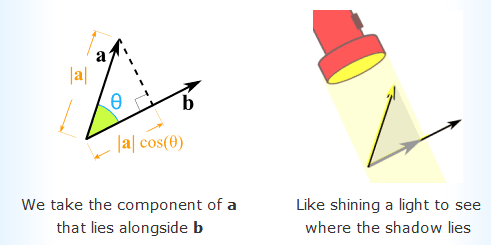
\includegraphics[width=0.5\linewidth]{vecproj}
\end{center}
If vectors are at right angles?
\tiny{(Reference: https://www.mathsisfun.com/algebra/vectors-dot-product.html)}
\end{frame}


%%%%%%%%%%%%%%%%%%%%%%%%%%%%%%%%%%%%%%%%%%%%%%%%%%%%%%%%%%%%%%%%%%%%%%%%
\begin{frame}[fragile]\frametitle{Dot Product}
\begin{itemize}
\item  The dot product of two vectors is the sum of their component-wise products. 
\item Hint: Similar to \lstinline|vector_add| but with a difference in return type
\end{itemize}
\begin{lstlisting}
def dot(v, w):
	:
	return ...
vv = [ 1, 2,3]
ww = [3,2,1]
result = dot(vv,ww)
print("Dot Product {}".format(result))
\end{lstlisting}
\end{frame}

%%%%%%%%%%%%%%%%%%%%%%%%%%%%%%%%%%%%%%%%%%%%%%%%%%%%%%%%%%%%%%%%%%%%%%%%
\begin{frame}[fragile]\frametitle{Dot Product}
Solution:
\begin{lstlisting}
def dot(v, w):
    """v_1 * w_1 + ... + v_n * w_n"""
    return sum(v_i * w_i
               for v_i, w_i in zip(v, w))
\end{lstlisting}
Dot Product 10.
%%\end{frame}
%%
%%%%%%%%%%%%%%%%%%%%%%%%%%%%%%%%%%%%%%%%%%%%%%%%%%%%%%%%%%%%%%%%%%%%%%%%%%
%%\begin{frame}[fragile]\frametitle{Dot Product}
%%Its a projection
%%\begin{center}
%%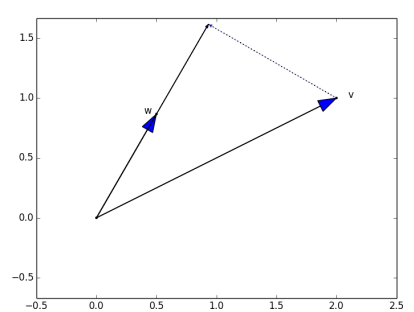
\includegraphics[width=0.5\linewidth]{vecdot}
%%\end{center}

Easy to compute a vector's sum of squares:
\begin{lstlisting}
def sum_of_squares(v):
    """v_1 * v_1 + ... + v_n * v_n"""
    return dot(v, v)
\end{lstlisting}
\end{frame}

%%%%%%%%%%%%%%%%%%%%%%%%%%%%%%%%%%%%%%%%%%%%%%%%%%%%%%%%%%%%%%%%%%%%%%%%%%
%%\begin{frame}[fragile]\frametitle{Dot Product}
%%Easy to compute a vector's sum of squares:
%%\begin{lstlisting}
%%def sum_of_squares(v):
%%    """v_1 * v_1 + ... + v_n * v_n"""
%%    return dot(v, v)
%%\end{lstlisting}
%%\end{frame}

%%%%%%%%%%%%%%%%%%%%%%%%%%%%%%%%%%%%%%%%%%%%%%%%%%%%%%%%%%%%%%%%%%%%%%%%
\begin{frame}[fragile]\frametitle{Magnitude of a Vector}
\begin{lstlisting}
import math
def magnitude(v):
    return math.sqrt(sum_of_squares(v)) 
\end{lstlisting}
\end{frame}

%%%%%%%%%%%%%%%%%%%%%%%%%%%%%%%%%%%%%%%%%%%%%%%%%%%%%%%%%%%%%%%%%%%%%%%%
\begin{frame}[fragile]\frametitle{Distance Between Vectors}
\begin{itemize}
\item  Formula:
$ \sqrt{(v_1 - w_1)^2 + \ldots (v_n - w_n)^2}$
\item Hint: First use \lstinline|vector_subtract| and then \lstinline|sum_of_squares|
\item For now, do not bother about normalizing it with product of their magnitudes.

\end{itemize}
\begin{lstlisting}
def squared_distance(v, w):
	:
	return ...
vv = [ 1, 2,3]
ww = [3,2,1]
result = squared_distance(vv,ww)
print("Squared Distance {}".format(result))
\end{lstlisting}
\end{frame}

%%%%%%%%%%%%%%%%%%%%%%%%%%%%%%%%%%%%%%%%%%%%%%%%%%%%%%%%%%%%%%%%%%%%%%%%
\begin{frame}[fragile]\frametitle{Distance}

\begin{lstlisting}
def squared_distance(v, w):
    """(v_1 - w_1) ** 2 + ... + (v_n - w_n) ** 2"""
    return sum_of_squares(vector_subtract(v, w))
    
def distance(v, w):
   return math.sqrt(squared_distance(v, w))
\end{lstlisting}
or
\begin{lstlisting}
def distance(v, w):
    return magnitude(vector_subtract(v, w))
\end{lstlisting}
Squared Distance 8
\end{frame}

%%%%%%%%%%%%%%%%%%%%%%%%%%%%%%%%%%%%%%%%%%%%%%%%%%%%%%%%%%%%%%%%%%%%%%%%
\begin{frame}[fragile]\frametitle{Matrices}
\begin{itemize}
\item  A matrix is a two-dimensional collection of numbers. 
\item list of  lists, with each inner list having the same size and representing a row of the
matrix.
\item  If  $A$  is a matrix, then  $A[i][j]$  is the element in the $i$th row and the $j$th column.
\end{itemize}
\begin{lstlisting}
A = [[1, 2, 3],  # A has 2 rows and 3 columns
     [4, 5, 6]]
B = [[1, 2],     # B has 3 rows and 2 columns
     [3, 4],
     [5, 6]]
\end{lstlisting}
\end{frame}

%%%%%%%%%%%%%%%%%%%%%%%%%%%%%%%%%%%%%%%%%%%%%%%%%%%%%%%%%%%%%%%%%%%%%%%%
\begin{frame}[fragile]\frametitle{Matrices}
\begin{itemize}
\item  Python lists, being `0' indexed, first row of a matrix ``row 0'' and the first column ``column 0''.
\item  matrix  $A$  has  $len(A)$  rows and  $len(A[0])$ columns, which we consider its  shape
\end{itemize}
\begin{lstlisting}
def shape(A):
    num_rows = len(A)
    num_cols = len(A[0]) if A else 0 
    return num_rows, num_cols
\end{lstlisting}
Numpy and Pandas Dataframes have in built matrix functionality needed for Data Science
\end{frame}
